\documentclass{article}
\usepackage[utf8]{inputenc}
\usepackage[a4, margin=20mm]{geometry}
\usepackage{pgfplots}
\usepackage{graphicx}
\graphicspath{ {./img/} }


\title{Wirtschaftsstatistik - ESA 1}
\author{Przemyslaw Jozwiak - Matrikelnummer 885582}
\date{07. November 2020}


\begin{document}

\maketitle
\newpage


\section*{Aufgabe 1}
\section{Teil A}
Um die Auswirkung der Regelstudienzeit zu demonstrieren, wurden die Studienzeiten von 200 Wirtschaftsingenieuren erhoben, die in den vergangenen vier Semestern ihr Studium erfolgreich abgeschlossen haben.
Es ergaben sich folgende (fiktive) Daten:

\begin{center}
\begin{tabular}{| c | c | c | c | c | c | c | } 
\hline
Semesterzahl & 10 & 11 & 12 & 13 & 14 & 15 \\ 
\hline
relative Häufigkeiten & 0,1 & 0,1 & 0,4 & 0,2 & 0,15 & 0,05 \\ 
\hline
\end{tabular}
\end{center}

\subsection{Wie heißt die statistische Größe (Merkmal) und wie ist es skaliert?}
Semesterzahl ist hier uns Merkmal und es ist diskret.

\subsection{Bestimmen Sie die absoluten Häufigkeiten (Häufigkeitstabelle).}
\begin{center}
\begin{tabular}{| c | c | c | c | c | c | c | } 
\hline
Semesterzahl & 10 & 11 & 12 & 13 & 14 & 15 \\ 
\hline
absolute Häufigkeiten & 20 & 20 & 80 & 40 & 30 & 10 \\ 
\hline
\end{tabular}
\end{center}

\subsection{Bestimmen Sie die absoluten und relativen kumulierten Häufigkeiten.}
\begin{center}
\begin{tabular}{| c | c | c | c | c | c | c | } 
\hline
Semesterzahl & 10 & 11 & 12 & 13 & 14 & 15 \\ 
\hline
absolute Häufigkeiten & 20 & 20 & 80 & 40 & 30 & 10 \\ 
\hline
relative Häufigkeiten & 0,1 & 0,1 & 0,4 & 0,2 & 0,15 & 0,05 \\
\hline
absolute kumulierte Häufigkeit & 10 & 10 + 11 = 21 & 21 + 12 = 33 & 33 + 13= 46 & 46 + 14= 60 & 60 + 15 = 75\\
\hline
relative kumulierte Häufigkeit & 0,1 & 0,1+ 0,1= 0,2 & 0,2+ 0,4= 0,6 & 0,6+ 0,2= 0,8 & 0,8+ 0,15= 0,95 & 0,95+ 0,05= 1\\
\hline
\end{tabular}
\end{center}

\subsection{Skizzieren Sie (Graph) die relative Häufigkeitsfunktion und Verteilungsfunktion der statistischen Größe [absolut und relativ].}


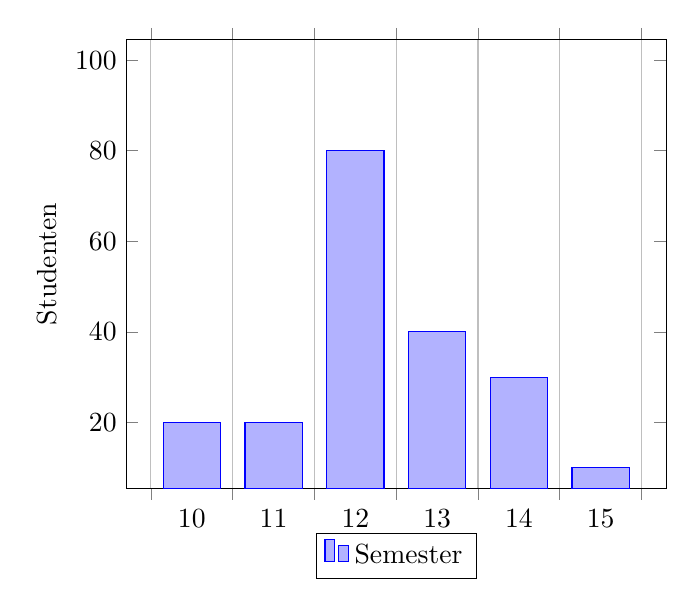
\begin{tikzpicture}
\begin{axis}[
	x tick label style={
		/pgf/number format/1000 sep=},
	ylabel=Studenten,
	enlargelimits=0.05,
	legend style={at={(0.5,-0.1)},
	anchor=north,legend columns=-1},
	ybar interval=0.7,
]
\addplot 
	coordinates {(15,10) (14,30) (13,40) (12,80) (11,20) (10,20) (9,100)};
\legend{Semester}
\end{axis}
\end{tikzpicture}


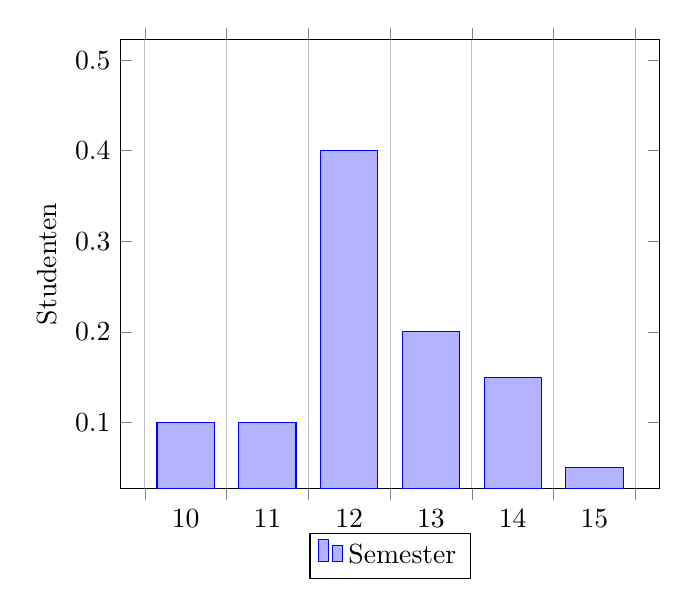
\begin{tikzpicture}
\begin{axis}[
	x tick label style={
		/pgf/number format/1000 sep=},
	ylabel=Studenten,
	enlargelimits=0.05,
	legend style={at={(0.5,-0.1)},
	anchor=north,legend columns=-1},
	ybar interval=0.7,
]
\addplot 
	coordinates {(15,0.05) (14,0.15) (13,0.2) (12,0.4) (11,0.1) (10,0.1) (9,0.5)};
\legend{Semester}
\end{axis}
\end{tikzpicture}

\subsection{Wie viele Semester höchstens benötigen die 10\% schnellsten Studenten?}
Die schnellsten 10\% aller der 200 Studenten benötigen 10 Semester.

\subsection{Wie viele Semester mindestens benötigen die 80\% langsamsten Studenten?}
Die langsamen 80\% der Studenten benötigen zwischen 12 und 15 Semester.

\subsection{Geben Sie die Semesterzahl an, die genau 20\% der Studenten benötigen}
Die Anzahl der Semester, die 20\% der Studenten benötigen, beträgt 13.

\section{Teil B}
Im Teil B soll nur noch das Merkmal Y: "Semesterzahl" mit den Ausprägungen:

\begin{tabular}{ l l  } 
"klein" & (weniger als 12 Semester)\\
"mittel" & (genau 12 Semester)\\
"groß" & (mehr als 12 Semester)
\end{tabular}\\
betrachtet werden.

\subsection{Welche Skalierungsart liegt jetzt vor?}
Hier liegt eine Ordinalskala vor.

\subsection{Stellen Sie die absolute (nur) Häufigkeitsfunktion auf (Tabelle + Graph).}
\begin{center}
\begin{tabular}{| c | c | c | c | } 
\hline
"Semesterzahl" & "klein" & "mittel" & "groß" \\ 
\hline
absolute Häufigkeiten & 40 & 80 & 80 \\ 
\hline
\end{tabular}
\end{center}

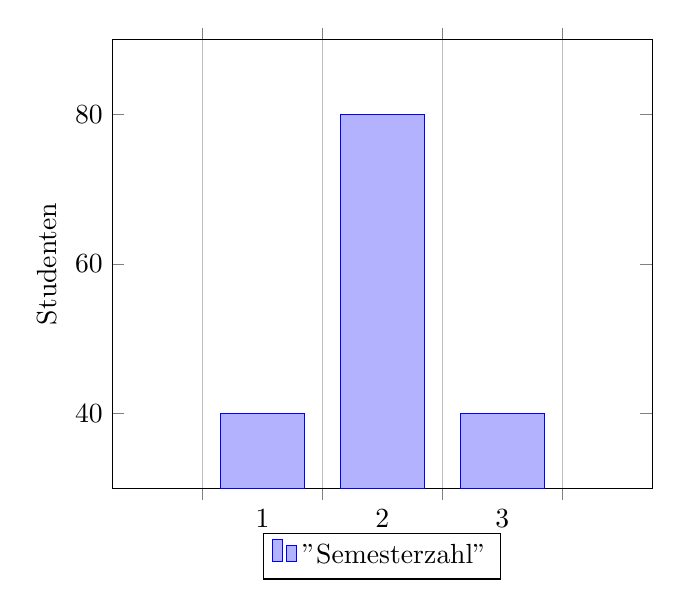
\begin{tikzpicture}
\begin{axis}[
	x tick label style={
		/pgf/number format/1000 sep=},
	ylabel=Studenten,
	enlargelimits=0.25,
	legend style={at={(0.5,-0.1)},
	anchor=north,legend columns=-1},
	ybar interval=0.7,
]
\addplot 
	coordinates {(1,40) (2,80) (3,40) (4,80)};
\legend{"Semesterzahl"}
\end{axis}
\end{tikzpicture}

\subsection{Ist es sinnvoll, bei einem nominal skalierten Merkmal eine Verteilungsfunktion
anzugeben? [Begründen Sie]}
Nein, dies ist nicht sinnvoll da die Werte einer Nominalskala, da wir die sich die Werte zwar unterscheiden aber wir diese nicht sortieren können.

\section{Aufgabe 2}
Ein Sportverein hat sich in seiner Leichtathletikabteilung einen Schwerpunkt in der Förderung des 100-Meter-Laufs gesetzt.
Nach einem Jahr intensivsten Trainings wurden die Zeiten der 20 Läufer des Vereins gemessen. Dabei ergab sich folgende Verteilungsfunktion:\\
\includegraphics{aufg2_grph.png}

\subsection{Zeichnen Sie das zur Verteilungsfunktion gehörende Histogramm.}

\begin{center}
\begin{tabular}{ | c | c | c | c | c | } 
\hline
Läufer & 10.2 & 10.6 & 10.8 & 11\\
\hline
relative Häufigkeit & 0.1 & 0.5 & 0.2 & 0.2 \\
\hline
absolute Häufigkeit & 2 & 10 & 4 & 4\\
\hline
\end{tabular}
\end{center}

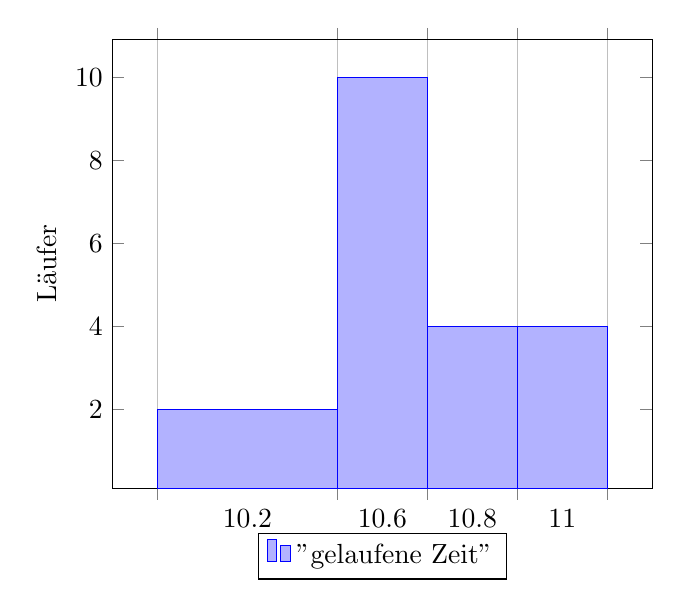
\begin{tikzpicture}
\begin{axis}[
	x tick label style={
		/pgf/number format/1000 sep=},
	ylabel=Läufer,
	enlargelimits=0.1,
	legend style={at={(0.5,-0.1)},
	anchor=north,legend columns=-1},
	ybar interval=1,
]
\addplot 
	coordinates {(10.2,2) (10.6,10) (10.8,4) (11,4) (11.2,1)};
\legend{"gelaufene Zeit"}
\end{axis}
\end{tikzpicture}

\subsection{Welche Zeit höchstens benötigen die 80\% schnellsten Läufer?}
Die schnellsten 80\% der Läufer benötigen 10,8 Sekunden.

\end{document}
